\documentclass{article}
%hvem faen er krampedunk?
% \documentclass[aps,rmp,reprint,amsmath,amssymb,graphicx,longbibliography]{article}
\usepackage[utf8]{inputenc}
\usepackage{graphicx}
\usepackage{float}
\usepackage{listings}
\usepackage{amsmath}
\usepackage{amssymb}
\usepackage{mathtools}
\usepackage{commath}
\usepackage{tabularx}
\usepackage[ruled,vlined]{algorithm2e}
\graphicspath{{./plots/}}
% \usepackage{biblatex}
% \addbibresource{refs.bib}
\usepackage{caption}
\usepackage{subcaption}
\usepackage{minted}

% \usepackage{longbibliography}

\bibliographystyle{apalike}
\usepackage{hyperref}
\hypersetup{breaklinks=true,colorlinks=true,linkcolor=blue,citecolor=blue,filecolor=magenta,urlcolor=blue}

\DeclareMathOperator*{\argmax}{arg\,max}
\DeclareMathOperator*{\argmin}{arg\,min}
\DeclareMathOperator*{\sgn}{sgn}
\DeclareMathOperator*{\Bias}{Bias}
\DeclareMathOperator*{\Var}{Var}

\title{Regression analysis and resampling methods applied to the Franke's Function}
\author{Femtehjell, Hoel, Otterlei and Steeneveldt}

\date{September 2023}

% Sample for adding code to text:
% \inputminted[frame=lines,
% framesep=2mm,
% linenos,
% fontsize=\footnotesize]{python}{filename.py}

\def\@bibdataout@aps{%
\immediate\write\@bibdataout{%
@CONTROL{%
apsrev41Control%
\longbibliography@sw{%
    ,author="08",editor="1",pages="1",title="0",year="1"%
    }{%
    ,author="08",editor="1",pages="1",title="",year="1"%
    }%
  }%
}%
\if@filesw \immediate \write \@auxout {\string \citation {apsrev41Control}}\fi
}

\begin{document}


\maketitle
\begin{figure}[H]
    \centering
    
\includegraphics[scale=0.5]{Project1/1797261_uio-logo.png}
\end{figure}
\newpage
\tableofcontents
\newpage

\section*{Abstract}

In this project, we aim to gain valuable insights from a dataset of terrain data using various regression methods such as Ordinary Least Squares (OLS), Ridge, and LASSO. To achieve this, we utilize two-variable polynomials at varying orders and carefully tune hyperparameters such as $\lambda$ for Ridge and LASSO methods. Additionally, we employ advanced resampling techniques such as non-parametric bootstrap and k-fold cross-validation. These techniques help us accurately assess the models' performance by dividing the data into test and training subsets and evaluating the performance multiple times by training the model with the training subset and evaluating with the testing subset.

To measure the performance of our regression methods, we use well-established metrics such as Mean Squared Error (MSE) and R2 score. Initially, we validate the methods on a well-known smooth function, the Franke function with Gaussian noise, before adapting and re-tuning the same methods for the more complicated terrain data. Our analysis reveals that Ridge regression provides the best fit for the terrain data.

\section{Introduction}
Machine learning has become wildly popular in the last decade. It is now used to some degree in all aspects of society and keeps growing in popularity. The most popular of the different machine learning models are deep learning, which is based on neural network and the base layer of neural networks theory is regression methods. This project will look into the theory of different regression methods and re-sampling techniques. Specifically, the project will look how to use linear regression, ridge and lasso regression to model polynomials of different degrees and how they differ in output.

Early in our education, we learn how to connect points by drawing a straight line through them. However, when such a line does not exists, how should one proceed? You may perhaps try to draw a wave through the points, or maybe draw a straight line through which is the 'closest' to all the points. Later we learn how to utilize tools to automatically create these lines, which are as mathematically close to the points as possible, but how does this work? How does the computer decide which type of line to draw, and how does it calculate how 'far' the line is from the points?

Suppose all of your points lay along a line, except one which is far away. Should the best line be the one which passes straight through most of the points, or should we penalize it for being far from one of the points. Maybe we should draw a line which goes straight from point to point, deviating far to catch the deviant. What if we know that we only have a handful of all the points, and that we want to place the line such that future points will also lay close to it. Does your answer change then?

We find the answers to these questions within the art of regression. One common way to calculate the deviation of points from the line, is to calculate the mean sum of the square of the errors (MSE), a method often attributed to Galileo Galilei \cite{galileo}. This method is what we find at the core of our first regression method, namely ordinary least squares (OLS), which tries to minimize this metric. This however, may cause problems where our model is too closely fitted our line, such that new points lay far away. In order to alleviate some of these issues, there are more complex methods such as ridge and Lasso regression, which build on OLS, which add a penalty in order to make sure that the most relevant aspects of the line are prioritized.

We will apply these methods to the Franke function, a method commonly used to test interpolation problems \cite{Franke:1982}. This function consists of two peaks, which is ideal as we will later attempt to analyse real world terrain data.

\section{Theory}
Linear regression is a well-known and well-used method in statistics. It is the method of drawing a line through a set of data to match the data points best as possible. It creates a
\begin{equation*}
    y = f(x) + \epsilon
\end{equation*}
where $y$ are the resulting values, $f(x)$ is the function we want to approximate and $\epsilon$ is the error estimate. For a single dimension, this becomes
\begin{equation*}
    y = \beta x + \epsilon
\end{equation*}
When fitting this to data, this will look like this
%%%%
% Insert linear regression plot w/o intercept
%%%%
As we can see from the plot, this does not work so well if the data is not naturally formed around the origin. To fix this we can add in a constant, called intercept, $\beta$. This gives us the equation
\begin{equation*}
    y = \beta_0 + \beta_1x + \epsilon
\end{equation*}
From the figure below, we can see that this fits better as the intercept controls the starting point of the linear regression line.
%%%%
%% Add regression plot with intercept
%%%%
For the case in this project, we need to use linear regression in multiple dimensions. For this, we need to move to matrix calculus. Our new equation for linear regression becomes
\begin{equation*}
    \mathbf{y} = f(\mathbf{x}) + \mathbf{\epsilon}
\end{equation*}
where $\mathbf{x} = [x_1, x_2, x_3, ..., x_n]^T$. Since we can't know the original function $f$, we have to be satisfied with an approximation, which gives us
\begin{equation*}
    \mathbf{\Tilde{y}} = \mathbf{X\beta}
\end{equation*}
here, $\mathbf{X}$ is the design matrix and $\mathbf{\beta}$ is the weights

\newpage
\subsection{Ordinary Least Squares}
In order to have a basis to work from, we assume that there exists a continuous function $f: X \to Y$ such that our data points $\boldsymbol{y} \in Y$ can be described as
\begin{equation*}
    \boldsymbol{y} = f(\boldsymbol{x}) + \boldsymbol{\varepsilon},
\end{equation*}
where $\boldsymbol{\varepsilon} \sim N(0, \sigma^2)$. We are then looking for an approximation of $f$ which gives $\tilde{\boldsymbol{y}}$ such that the MSE $\frac{1}{n} \left( \boldsymbol{y} - \tilde{\boldsymbol{y}} \right)^2$ is minimized. In order to approximate $f$, we consider $n$ samples of $\boldsymbol{y}$ and assume that there are $p$ characteristics which define each of the samples, such that $y_i = f(\boldsymbol{x}_i) + \varepsilon_i$ where $\boldsymbol{x}_i = \left[x_{i,0}, x_{i, 1}, \ldots, x_{i, p-1} \right]$.

We gather this information in a matrix $\boldsymbol{X}$, called the design matrix, such that
\begin{equation*}
    \boldsymbol{X} =
    \begin{bmatrix}
        x_{0,0} & x_{0,1} & \ldots & x_{0, p-1} \\
        x_{1,0} & x_{1,1} & \ldots & x_{1, p-1} \\
        \vdots & \vdots & \ddots & \vdots \\
        x_{n,0} & x_{n,1} & \ldots & x_{n, p-1}
    \end{bmatrix}.
\end{equation*}
We are seeking to find a causal relationship between $\boldsymbol{y}$ and $\boldsymbol{x}$, and as we have no knowledge of what type of function $f$ is, we assume there is a linear relationship such that $y_i = \boldsymbol{x}_i \cdot \boldsymbol{\beta} + \varepsilon_i$, for some weight $\beta_i$. This can be written as
\begin{equation*}
    \boldsymbol{y} = \begin{bmatrix}
        x_{0,0} & x_{0,1} & \ldots & x_{0, p-1} \\
        x_{1,0} & x_{1,1} & \ldots & x_{1, p-1} \\
        \vdots & \vdots & \ddots & \vdots \\
        x_{n,0} & x_{n,1} & \ldots & x_{n, p-1}
    \end{bmatrix}
    \begin{bmatrix}
        \beta_0 \\ \beta_1 \\ \vdots \\ \beta_{p-1}
    \end{bmatrix}
    +
    \begin{bmatrix}
        \varepsilon_0 \\ \varepsilon_1 \\ \vdots \\ \varepsilon_{n}
    \end{bmatrix}
    = \boldsymbol{X} \boldsymbol{\beta} + \boldsymbol{\varepsilon},
\end{equation*}
where $f(\boldsymbol{x})$ is now equal to $\boldsymbol{X\beta}$. Our approximation $\boldsymbol{\tilde{y}}$ then becomes $\boldsymbol{\tilde{y}} = \boldsymbol{X\beta}$.

We call $\boldsymbol{x}_i$ the explanatory variables, $\boldsymbol{\beta}$ the regression parameter, and $\boldsymbol{y}$ the response variable.

Our goal is now to find $\boldsymbol{\hat{\beta}}$ such that $\left( \boldsymbol{y} - \boldsymbol{\tilde{y}} \right)^2$ is minimized, i.e.,
\begin{equation*}
    \boldsymbol{\hat{\beta}}  = \argmin_{\boldsymbol{\beta} \in \mathbb{R}^p} \frac{1}{n} \left( \boldsymbol{y} - \boldsymbol{X\beta} \right)^2 = \argmin_{\boldsymbol{\beta} \in \mathbb{R}^p} \frac{1}{n} \left( \boldsymbol{y} - \boldsymbol{X\beta} \right)^T \left( \boldsymbol{y} - \boldsymbol{X\beta} \right).
\end{equation*}
As then
\begin{equation*}
    \left( \boldsymbol{y} - \boldsymbol{X\beta} \right)^T \left( \boldsymbol{y} - \boldsymbol{X\beta} \right) = \boldsymbol{y}^T \boldsymbol{y} - 2 \boldsymbol{\beta}^T \boldsymbol{X}^T \boldsymbol{y} + \boldsymbol{\beta}^T \boldsymbol{X}^T \boldsymbol{X} \boldsymbol{\beta} 
\end{equation*}
is a non-negative quadratic equation, the minimum must exist. We may therefore find it by equating the partial derivatives with respect to the $p$ components of $\boldsymbol{\beta}$ with zero. In finding the derivative, we can ignore the scaling factor $\frac{1}{n}$

\begin{gather*}
    \frac{\partial}{\partial \boldsymbol{\beta}} \left( \boldsymbol{y}^T \boldsymbol{y} - 2 \boldsymbol{\beta}^T \boldsymbol{X}^T \boldsymbol{y} + \boldsymbol{\beta}^T \boldsymbol{X}^T \boldsymbol{X} \boldsymbol{\beta} \right) = 0 \\
    -2 \boldsymbol{X}^T \boldsymbol{y} + 2 \boldsymbol{X}^T \boldsymbol{X \beta} = 0 \\
    2 \boldsymbol{X}^T \boldsymbol{X \beta} = 2 \boldsymbol{X}^T \boldsymbol{y} \\
    \boldsymbol{\beta} = \left( \boldsymbol{X}^T \boldsymbol{X} \right)^{-1} \boldsymbol{X}^T \boldsymbol{y}
\end{gather*}

When the matrix $\boldsymbol{X}^T \boldsymbol{X}$ is invertible, this solution $\boldsymbol{\hat{\beta}}$ which minimizes the MSE can be found precisely. Often, especially when working numerically, the matrix is singular, so we instead apply the Moore-Penrose generalised inverse defined from the Singular Value Decomposition, often just called the pseudoinverse \cite[p.~74--82]{introNumeric}.


\subsubsection{Single Value Decomposition}
% Maybe move this down after Lasso?
When $\mathbf{X}^T\mathbf{X}$ is not invertible, we can solve this using the method of the SVD algorithm. SVD is defined as
\begin{equation*}
    \mathbf{A} = \mathbf{U}\mathbf{\Sigma}\mathbf{V}^T
\end{equation*}

\subsection{Ridge}
When conducting Ordinary Least Squares (OLS) regression, overfitting can be a challenge. Overfitting occurs when our model closely conforms to the training data, not only capturing the genuine underlying pattern but also incorporating the random fluctuations present in our data. This can result in a model that exhibits exceptional performance on the training data it has seen but performs poorly when tasked with predicting unseen data.

Overfitting is influenced by two closely related factors: the density of our training data and the complexity of our model. Ideally, with an infinitely dense training dataset, we could employ an arbitrarily complex model. Acquiring such a dataset is in practice often impossible%There is a regression technique called k-nearest neighbors suited for such a purpose 
. Our model must therefore deliver reliable performance even when trained on a limited number of data points.

% However, acquiring such an extensive dataset is often impractical, not to mention that even if obtained regression would then be inefficient for predictive purposes. Therefore, our model must strike a balance, delivering reliable performance even when trained on a limited number of data points.

Ridge regression is a method which aims to address this by taking into account the size of the values in the regression parameter $\boldsymbol{\beta}$. The cost function is now defined as
\begin{align*}
    C \left( \boldsymbol{X}, \boldsymbol{\beta} \right) &= \frac{1}{n} \lVert\boldsymbol{y} - \boldsymbol{\tilde{y}} \rVert_2^2 + \lambda \lVert \boldsymbol{\beta} \rVert_2^2 \\
    &= \frac{1}{n} \left( \boldsymbol{y} - \boldsymbol{X\beta} \right)^2 + \lambda \boldsymbol{\beta}^2
\end{align*}

% Ridge regression is a method which aims to address this by utilizing the cost function
% \begin{align*}
%     C(\boldsymbol{X},\boldsymbol{\beta})=&\frac{1}{n}\vert\vert \boldsymbol{y}-\boldsymbol{\tilde{y}}\vert\vert_2^2+\lambda\vert\vert \boldsymbol{\beta}\vert\vert_2^2\\
%     =& \frac{1}{n}\vert\vert \boldsymbol{y}-\boldsymbol{X}\boldsymbol{\beta}\vert\vert_2^2+\lambda\vert\vert \boldsymbol{\beta}\vert\vert_2^2
% \end{align*}

The right addend ($\lambda\lVert \boldsymbol{\beta} \rVert_2^2$) is called the regularization term, and we require that $\lVert \boldsymbol{\beta} \rVert_2^2 \leq t$ for some finite constant $t > 0$. It penalizes large regression coefficients, discouraging the model from assigning excessive importance to any single feature. This skews our predictions closer to zero. Resulting in higher bias, but lower variance.

The strength of the regularization is determined by $\lambda$. When $\lambda=0$, we recover OLS regression. By increasing the value of the hyperparameter $\lambda$, we enforce stronger penalization on large coefficient values, effectively skewing our predictions more towards zero. The optimal value of $\lambda$ can be determined through resampling techniques.

Given a $\lambda$ our optimal regression parameter $\boldsymbol{\hat{\beta}}$ minimizes the cost function. That is
% \begin{equation*}
%     \frac{1}{n} \left( \boldsymbol{y} - \boldsymbol{X} \boldsymbol{\hat{\beta}} \right)^2 + \lambda \boldsymbol{\hat{\beta}}^2 = \min_{\boldsymbol{\beta} \in \mathbb{R}^p} \frac{1}{n} \left( \boldsymbol{y} - \boldsymbol{X} \boldsymbol{\beta} \right)^2 + \lambda \boldsymbol{\beta}^2
% \end{equation*}
\begin{equation*}
    \boldsymbol{\hat{\beta}} = \argmin_{\boldsymbol{\beta} \in \mathbb{R}^p} \frac{1}{n} \left( \boldsymbol{y} - \boldsymbol{X} \boldsymbol{\beta} \right)^2 + \lambda \boldsymbol{\beta}^2
\end{equation*}
The right hand side multiplies out to
\begin{equation*}
    \frac{1}{n} \left( \boldsymbol{y}^T \boldsymbol{y} - 2 \boldsymbol{\beta}^T \boldsymbol{X}^T \boldsymbol{y} + \boldsymbol{\beta}^T \boldsymbol{X}^T \boldsymbol{X} \boldsymbol{\beta} \right) + \lambda \boldsymbol{\beta}^T \boldsymbol{\beta},
\end{equation*}
which again is a non-negative quadratic, meaning the minimum exists. We proceed similarly as with OLS, by taking the partial derivatives with respect to each component of $\boldsymbol{\beta}$ and equating it with zero. As $\frac{1}{n}$ is just a scaling factor, we can safely ignore it while finding the derivative.
\begin{gather*}
    \frac{\partial}{\partial \boldsymbol{\beta}} \left( \left( \boldsymbol{y} - \boldsymbol{X} \boldsymbol{\beta} \right)^2 + \lambda \boldsymbol{\beta}^2 \right) = 0 \\
    -2 \boldsymbol{X}^T \boldsymbol{y} + 2 \boldsymbol{X}^T \boldsymbol{X \beta} + 2\lambda \boldsymbol{\beta} = 0 \\
    \boldsymbol{X}^T \boldsymbol{X \beta} + \lambda \boldsymbol{\beta} = \boldsymbol{X}^T \boldsymbol{y} \\
    \left(\boldsymbol{X}^T \boldsymbol{X} + \boldsymbol{I}_p \lambda \right) \boldsymbol{\beta} = \boldsymbol{X}^T \boldsymbol{y} \\
    \boldsymbol{\beta} = \left(\boldsymbol{X}^T \boldsymbol{X} + \boldsymbol{I}_p \lambda \right)^{-1} \boldsymbol{X}^T \boldsymbol{y}
\end{gather*}

Again, we apply the pseudoinverse when finding $(\boldsymbol{X}^T \boldsymbol{X} + \lambda \boldsymbol{I})^{-1}$. This gives us that the optimal parameter $\boldsymbol{\hat{\beta}}$ for ridge regression is given by
\begin{equation*}
    \boldsymbol{\hat{\beta}}_\text{Ridge} = (\boldsymbol{X}^T \boldsymbol{X} + \lambda \boldsymbol{I})^{-1} \boldsymbol{X}^T \boldsymbol{y}.
\end{equation*} 




\subsection{Lasso}
LASSO is an abbreviation of Least Absolute Shrinkage and Selection Operator, and performs both regularization as in Ridge regression, and predictor selection.

Here, the cost function is defined as
\begin{align*}
    C \left( \boldsymbol{X}, \boldsymbol{\beta} \right) &= \frac{1}{n} \lVert \boldsymbol{y} - \boldsymbol{X\beta} \rVert_2^2 + \lambda \lVert \boldsymbol{\beta} \rVert_1 \\
    &= \frac{1}{n} \left( \boldsymbol{y} - \boldsymbol{X\beta} \right)^2 + \lambda \sum_i |\beta_i|.
\end{align*}
%Predictor selection happens when we add a constraint on the size of the penalty
To see why predictor selection happens with Lasso regression it's help full to have a look at a simple model with two features and two corresponding $\beta$ values
%\begin{align*}
 %   \lVert \boldsymbol{\beta} \rVert_1 \leq s, \hspace{10mm} 0\leq s
%\end{align*}
%such that the OLS solution is not within the space of suitable $\beta$. This is most easily explained by looking at a simpler model with two features and two corresponding $\beta$ values

% Chillern, tror jeg skjønner litt mer nå
%Hei jeg er også med :D
% Bildet er fra hastie et.al.! (sånn cirkus)
\begin{center}
    % 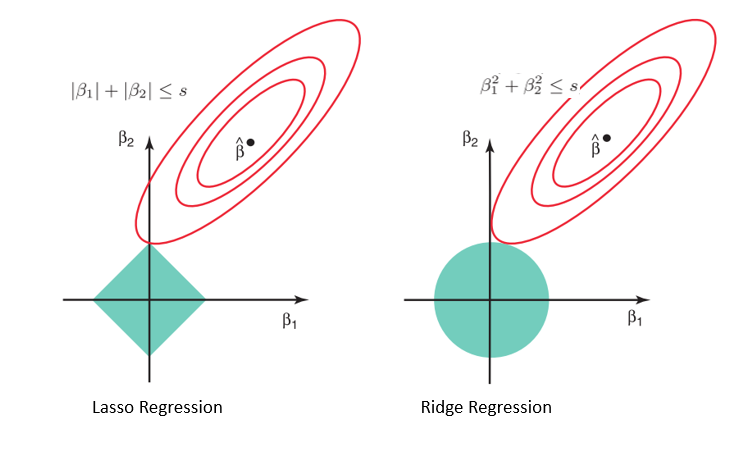
\includegraphics[width=95mm]{lasso_ridge_contour.png}
    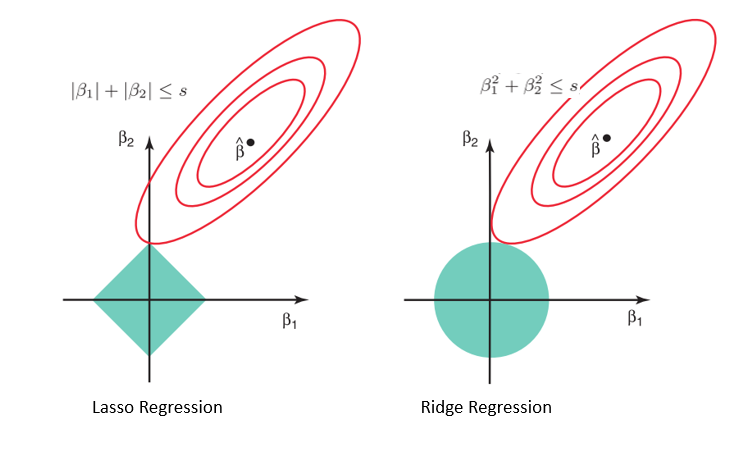
\includegraphics[width=\textwidth]{lasso_ridge_contour.png}
    % Include caption, figure num, source, ...
\end{center}


Here, $\boldsymbol{\hat{\beta}}$ is the OLS solution, along with the contour lines for for other values of $\boldsymbol{\beta}$. As we relax the constraint $s$, we grow the ``diamond" generated by the constrained $l_1$ norm until it meets with the target ellipse, and the corners of the diamond are more likely to intersect before the edges. This is especially the case when working higher dimensions, as the corners stick out further \cite[p.~432--436]{Murphy2012}. This is not the case with the constrained $l_2$ norm, as it has no ``corners" along the axes.

Due to the nature of the $l_1$ norm, there exists no neat analytical solution, as absolute values do not perform nicely during derivation. We get that
\begin{align*}
    \frac{\partial}{\partial \boldsymbol{\beta}} \left( \frac{1}{n} \left( \boldsymbol{y} - \boldsymbol{X\beta} \right)^2 + \lambda \sum_i |\beta_i| \right) &= 0 \\
    -2 \boldsymbol{X}^T \boldsymbol{y} + 2 \boldsymbol{X}^T \boldsymbol{X\beta} + \lambda \sgn(\boldsymbol{\beta}) &= 0 \\
    2 \boldsymbol{X}^T \boldsymbol{X\beta} + \lambda \sgn(\boldsymbol{\beta}) &= -2 \boldsymbol{X}^T \boldsymbol{y},
\end{align*}
which we've yet to find a closed, generalised, form of.

\subsection{Scaling}
Scaling data is an essential concept in regression modeling, particularly in regularized regression. The process involves adjusting the values of numeric features in your dataset to a common scale, ensuring each feature has comparable magnitudes.
This standardization or normalization of the features can prove highly beneficial in several ways.

One of the primary advantages of data scaling is in the realm of computational performance. As there exists no analytical solution for Lasso regression, we instead approximate it numerically. This is done through coordinate decent, which converges faster when the features are scaled.
%looking for source for the above statement. Explaining it seemd difficult

Another important advantage of scaling is the ease it brings in model interpretation. When the ranges of different features vary widely, it's hard to compare the weights that a model assigns to individual features. However, with scaling, the weights can be interpreted on a comparable basis, providing meaningful insights \cite[p.~237]{james2021introduction}.

To see how scale impacts the accuracy of regularized regression let $\boldsymbol{\hat{\beta}}$ denote the OLS solution to some design matrix X. Then multiply column $j$ in our design matrix by 1000. The value of $\hat{\beta}_j$ to our new OLS problem will have shrunk by the same factor of 1000. In these two problems the relationship between our response variable ($\boldsymbol{y}$) and explanatory variable ($X_j$) is the same, but regularized regression treat them very differently. As in the first case the penalty of including our explanatory variable is 1000 times larger \cite[p.~237]{james2021introduction}. Thus the importance of features with a small variance, but high predictive power will be underestimated, and features with large variance, but small predictive power will be overestimated.

Scaling is performed through the formula
\begin{equation*}
    \tilde{x}_{i,j} = \frac{x_{i,j}}{\sqrt{\frac{1}{n} \sum_{i=0}^{n-1} \left( x_{i,j} - \Bar{x}_j \right)^2 }},
\end{equation*}
where 
\begin{equation*}
    \bar{x}_j = \frac{1}{n} \sum_{i=0}^{n-1} x_{i,j}
\end{equation*}
is the mean value of the column. Thus, all of the scaled predictors will have a standard deviation of one \cite[p.~237]{james2021introduction}.
% Seksjon om SVD?

\subsection{Bias-Variance tradeoff}
In order to measure our models, we split our dataset into two difference sets. One for training, and one for testing. The variance of a model refers to the amount our approximation $\boldsymbol{\tilde{y}}$ would change for varying sets of training data, compared to the true value of $\boldsymbol{y}$ \cite[p.~34]{james2021introduction}. Ideally, we would not want our estimate of $\boldsymbol{\tilde{y}}$ to change too much based on our sample of training data.

The bias of a model refers to how our model handles the approximations necessary to work with a physical problem. Errors are generated when working with an idealised version of a problem, as we may be unable to capture the complexity present. A high bias indicates that our method is oversimplifying our data, in effect missing relevant features. This is called underfitting, where the model is too simple to capture patterns in the data.

The expected mean squared error of our model indicates how well we can expect the model to perform. It is defined as $\mathbb{E} \left[ (\boldsymbol{y} - \boldsymbol{\tilde{y}})^2 \right]$ \cite[p.~34]{james2021introduction}. As we assume that $\boldsymbol{y} = f(\boldsymbol{x}) + \boldsymbol{\varepsilon}$, we get that
\begin{align*}
    \mathbb{E} \left[ (\boldsymbol{y} - \boldsymbol{\tilde{y}})^2 \right] &=
    \mathbb{E} \left[ (f(\boldsymbol{x}) + \boldsymbol{\varepsilon} - \boldsymbol{\tilde{y}})^2 \right] \\
    &= \mathbb{E} \left[ \boldsymbol{\varepsilon}^2 \right] + \mathbb{E} \left[ \boldsymbol{\varepsilon} \right] \mathbb{E} \left[ f(\boldsymbol{x}) - \boldsymbol{\tilde{y}} \right] + \mathbb{E} \left[ (f(\boldsymbol{x}) - \boldsymbol{\tilde{y}})^2 \right] \\
    &= \sigma^2 + \mathbb{E}\left[ (f(\boldsymbol{x}) - \boldsymbol{\tilde{y}})^2 \right]
\end{align*}
Where we used that $\boldsymbol{\varepsilon} \sim N(0, \sigma^2)$, and $\Var[\boldsymbol{\varepsilon}] = \mathbb{E}\left[ \boldsymbol{\varepsilon}^2 \right] + \mathbb{E}[\boldsymbol{\varepsilon}]^2$, in the final step. Furthermore,
\begin{align*}
    \mathbb{E}\left[ (f(\boldsymbol{x}) - \boldsymbol{\tilde{y}})^2 \right] &= \mathbb{E}\left[ (f(\boldsymbol{x}) - \mathbb{E}[ \boldsymbol{\tilde{y}}] + \mathbb{E}[ \boldsymbol{\tilde{y}}] - \boldsymbol{\tilde{y}})^2 \right] \\
    \noalign{$= \mathbb{E}\left[ (f(\boldsymbol{x}) - \mathbb{E}[ \boldsymbol{\tilde{y}}])^2 \right] 
    + \mathbb{E}\left[ f(\boldsymbol{x}) - \mathbb{E}[ \boldsymbol{\tilde{y}}]\right] \mathbb{E}\left[ \mathbb{E}[ \boldsymbol{\tilde{y}}] - \boldsymbol{\tilde{y}} \right] 
    + \mathbb{E}\left[ (\mathbb{E}[ \boldsymbol{\tilde{y}}] - \boldsymbol{\tilde{y}})^2 \right]$}
    \intertext{As $\mathbb{E}\left[ \mathbb{E}[ \boldsymbol{\tilde{y}}] - \boldsymbol{\tilde{y}} \right] = \mathbb{E}[ \boldsymbol{\tilde{y}}] - \mathbb{E}[ \boldsymbol{\tilde{y}}] = 0$}
    &= \mathbb{E}\left[ (f(\boldsymbol{x}) - \mathbb{E}[ \boldsymbol{\tilde{y}}])^2 \right] 
    + \mathbb{E}\left[ (\boldsymbol{\tilde{y}} - \mathbb{E}[ \boldsymbol{\tilde{y}}])^2 \right] \\
    &= \Bias\left[ \boldsymbol{\tilde{y}} \right] + \Var\left[ \boldsymbol{\tilde{y}} \right]
\end{align*}
Combining this with our previous result gives us finally that
\begin{equation*}
    \mathbb{E}\left[ (\boldsymbol{y} - \boldsymbol{\tilde{y}})^2 \right] = \Bias\left[ \boldsymbol{\tilde{y}} \right] + \Var\left[ \boldsymbol{\tilde{y}} \right] + \sigma^2.
\end{equation*}

The $\sigma^2$ term is called the irreducible error \cite[p.~223]{Hastie2009}, and cannot be improved by our models. Ideally, we want to choose a method such that we have both low variance and low bias. However, typically as the complexity of our model increases, the variance increases. Conversely, the same applies in the other direction. As the complexity is decreased, we see a higher bias and a lower variance. This is called the Bias-Variance tradeoff \cite[p.~223]{Hastie2009}.

\subsection{Resampling}
Resampling methods allow us to repeatedly draw random samples from our training data, in order to learn more about our model. This allows us to better estimate the variance of the model, granting us information we would not have had, should we have trained on the entirety of our data at once. The two most commonly used methods of resampling is cross-validation and bootstrapping \cite[p.~197]{james2021introduction}.

\subsubsection{Cross-validation}
Cross-validation consists of splitting our initial dataset into multiple sets. To motivate this, we first consider the validation set approach. This consists of splitting our data into one training set, and one for testing or \textit{validation}. This allows us to estimate how well our model will perform after training on future data. Note that splitting our data can cause the estimated test error rate to vary widely, as we split our data randomly. It can also cause us to overestimate our test error, as models tend to perform better when trained on more data, and we are in this case only training on a subset of the total data we have available \cite[p.~198--200]{james2021introduction}.

When cross-validating, we attempt to alleviate some of these issues. One method is called Leave one out cross-validation (LOOCV), were we for each data point train the model on the remaining values, and then calculate the test error with the data point we left out. We then take the average of all of these values, giving us the LOOCV estimate. This is for most models quite computationally expensive, especially when we have a lot of data.

The upside of this method is that the mean squared error estimate were we excluded the observation $(x_i, y_i)$, where $\text{MSE}_i = (y_i - \tilde{y}_i)^2$, is approximately unbiased \cite[p.~201]{james2021introduction}. However, we expect a high variance as the training sets are so similar \cite[p.~242]{Hastie2009}.

A more sophisticated approach which alleviates some of the previous problems, is called K-Fold cross-validation. In this method, we split our data into $k$ roughly equal parts. We then reserve each fold as a validation set, training our model on the remaining $k-1$ folds. This has the benefit of being less computationally expensive, as we are only training our model $k$ times, while also having a lower variance. If our folds contain too few points, our model might suffer from high bias. We therefore typically choose either $k = 5$ or $k = 10$ as a compromise \cite[p.~243]{Hastie2009}.

\subsubsection{Bootstrapping}
Bootstrapping consists of generating new datasets by repeatedly drawing random values from our original data, with replacement. Each new dataset will be of the same size as the original. We generate $B$ datasets this way, refitting our model for each. We can then analyze how our model behaves for each of the datasets, allowing us to learn more about how our model performs. 

% Trenger mer

\subsection{Model evaluation and selection}


\newpage
\section{Method}
To begin testing the differences between the different regression methods and apply them to the topographic data, we first need a data set. This will make it easier to refine the implementation of the different regression methods. We first start by producing our own data set. To do this, we use Franke's function. A two-dimensional function often used for testing interpolation and fitting algorithms. It consists of two gaussian peaks, and is therefore apt for our use case. The function is defined as 
\begin{equation*}
    \begin{split}
        f(x,y) & = \frac{3}{4}\exp\left(-\frac{(9x-2)^2}{4} - \frac{(9y-2)^2}{4}\right) + \frac{3}{4}\exp\left(-\frac{(9x+1)^2}{49} - \frac{(9y+1)}{10}\right) \\
        & + \frac{1}{2}\exp\left(-\frac{(9x-7)^2}{4} - \frac{(9y-3)^2}{4}\right) - \frac{1}{5}\exp\left(-(9x-4)^2 - (9y-7)^2\right)
    \end{split}
\end{equation*}
where $x,y \in [0,1]$. To make the data more random, we add in some noise to the function, by drawing normally distributed values $\varepsilon \sim N(0,1)$. This gives us
\begin{equation*}
    z = f(x,y) + \alpha \cdot \varepsilon
\end{equation*}
where $\alpha$ is a constant such that $\alpha \in [0,1]$. Implemented in Python, $\boldsymbol{x}$, $\boldsymbol{y}$ and $\boldsymbol{\varepsilon}$ are all numpy arrays with length $n$.

As $f: [0,1] \times [0, 1] \to \mathbb{R}$ is a continuous function, and the set of all polynomials $\mathcal{P}$ is dense in $C([0,1] \times [0,1], \mathbb{R})$, we know by the Stone-Weierstrass Theorem that there exists a sequence of polynomials $\{p_n\}$ converging uniformly to $f$ \cite[p.~116--129]{lindstrom2017spaces}. In our case, this means that it is sensible to try to construct a polynomial which estimates our function $f$. As a polynomial function $p: \mathbb{R}^2 \to \mathbb{R}$ is a function
\begin{equation*}
    p(x,y) = \sum_{\substack{0 \leq n \leq N \\ 0 \leq m \leq M}} c_{n,m} x^n y^m,
\end{equation*}
we construct our explanatory variables $\boldsymbol{x}_i$ of all combinations $x_i^n y_i^m$ of $n,m \in \mathbb{N}$ such that $0 \leq n + m \leq N$ for some polynomial degree $N$. The regression parameter $\boldsymbol{\beta}$ then corresponds to the weights $c_{n,m}$.

The number of parameters for a polynomial degree of $N$ is then the sum of the combination for how many ways we can write $n+m = d$, for $0\leq n,m \leq d$, $d = 0, 1, \ldots, N$. We get
\begin{equation*}
    \text{\# $\boldsymbol{\beta}$ parameters} = \sum_{d = 0}^N \sum_{n = 0}^d 1
    = \sum_{d = 0}^N d + 1
    = \frac{(N + 1)(N + 2)}{2},
\end{equation*}
meaning that the complexity of our model increases quadratically as we increase the polynomial degree.

% På ridge, kan vi ikke bruke np.logspace for å lage lambdaene, sånn at vi får fin graf?
\section{Results}

\section{Discussion}

\section{Conclusion}

\section{References}

\bibliography{Project1/refs} % add  references to this 

\end{document}
